\documentclass{article}

\usepackage[czech]{babel}
\usepackage[a4paper,top=2cm,bottom=2cm,left=3cm,right=3cm,marginparwidth=1.75cm]{geometry}
\usepackage{amsmath}
\usepackage{graphicx}
\usepackage[colorlinks=true, allcolors=blue]{hyperref}

\title{Analýza dat}
\author{Tomáš Batelka}

\begin{document}
\maketitle

\section{Analýza dat}

\subsection{Analýza vstupních dat}

\begin{table}[h]
    \centering
    \begin{tabular}{r|l}
        Soubor & /home/vofy/Projects/pc2m-projekt/data/CntER.txt \\
        Počet záznamů & 115214l \\
        Celková doma měření & 115214 sekund
    \end{tabular}
    \caption{\label{tab:widgets}Analýza vstupních dat}
\end{table}

\subsection{Analýza hodnoty 3}

\begin{table}[h]
    \centering
    \begin{tabular}{r|l}
        Průměrná hodnota & 192.460314 \\
        Střední hodnota & 47.549000 \\
        Rozptyl & 73501.045098 \\
        Směrodatná odchylka & 271.110762 \\
        Integrál & 2757877.429530
    \end{tabular}
    \caption{\label{tab:widgets}Analýza hodnoty 3}
\end{table}


\section{Grafy}

\begin{figure}[h]
    \centering
    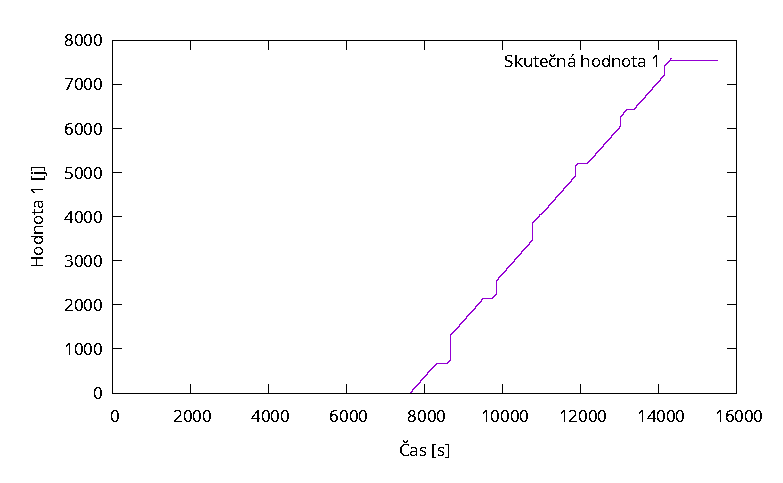
\includegraphics[]{plots/plot1.eps}
    \caption{\label{fig:plot1}Graf závislosti hodnoty 1 na čase}
\end{figure}

\begin{figure}[h]
    \centering
    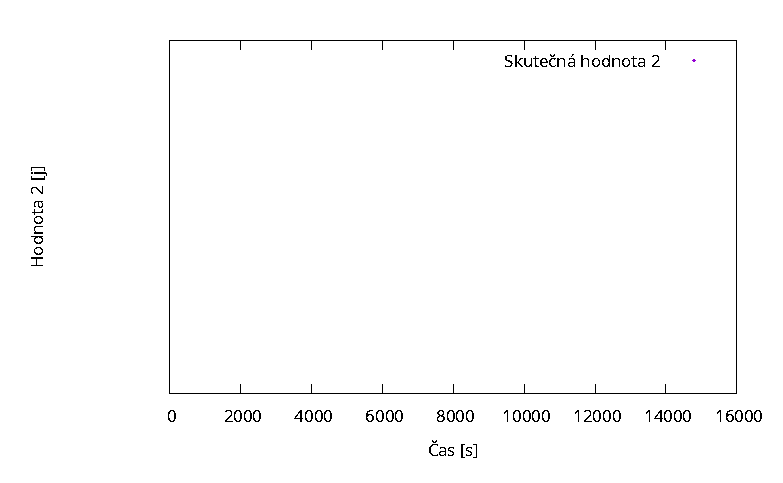
\includegraphics[]{plots/plot2.eps}
    \caption{\label{fig:plot2}Graf závislosti hodnoty 2 na čase}
\end{figure}

\begin{figure}[h]
    \centering
    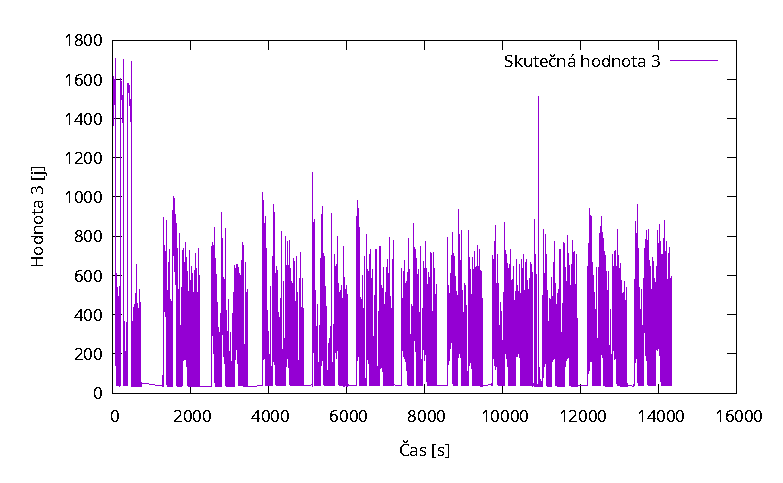
\includegraphics[]{plots/plot3.eps}
    \caption{\label{fig:plot3}Graf závislosti hodnoty 3 na čase}
\end{figure}

\end{document}